%=====================================================================
\section{Activity: does it enter only through $\la$?}\label{sec:activity}
H3: if activity entered only through $\la$, cavities with the same $R/\la$ would behave identically at any $\zeta$. Test at
$R=1.434\,\la$ (radius rescaled with the measured $\la(\zeta)$: $R=37.5$, 34.9, 31.8, 29.6, 27.3 for $\zeta=0.05$, 0.06, 0.07,
0.09, 0.11), $k=2\dots10$, 3 seeds. A bulk-sized patch of periodic box holds the same $\pi R^2/\la^2\approx6.5$ defects at
every activity.
\begin{table}[H]\centering\small
\caption{Activity scan at fixed $R/\la=1.43$ (site rule; ranges over $k=2\dots10$). Gap: $+\half$ density at $s\approx3$--4.5
relative to the bulk. Slope: $\mathrm{d}Q/\mathrm{d}s$ between $s=3$ and 5 ($k=8$), the flatness of the $+1$ plateau.}\label{tab:act}
\begin{tabularx}{\textwidth}{lccccccX}\toprule
$\zeta$ & $q_b$ & $P(q_b=+1)$ & pairs/frame & $\Phi$ & gap & slope & behaviour\\\midrule
0.05 & 1.16--1.81 & 0.36--0.68 & 0.6--1.3 & 0.83--0.92 ($k\le8$) & -- & -- & onset: vacant sites (e.g.\ $k=6$: 9.0 of 10), vortex fails at $k=9,10$\\
0.06 & 1.05--1.15 & 0.67--0.83 & 1.3--1.7 & 0.85--0.95 & shallow & 0.13 & mild onset\\
\textbf{0.07} & \textbf{1.01--1.09} & \textbf{0.89--0.96} & 1.5--2.0 & 0.89--0.97 & $\sim5\times$ & \textbf{0.07} & clean\\
0.09 & 1.01--1.05 & 0.77--0.92 & 1.9--2.4 & 0.88--0.99 & $\sim4\times$ & 0.15 & clean bulk; centre depleted\\
0.11 & 1.0--1.2 ($k\le6$) & 0.6--0.8 & 2.3 & 0.98 & $\sim1.5\times$ & 0.32 & gap closes; split ill-defined for $k\ge7$\\\bottomrule
\end{tabularx}
\end{table}
\begin{itemize}
  \item \textbf{$\zeta=0.05$ is the turbulence onset}: few dynamical defects (no pair in 22--50\% of frames against $\approx5\%$ at
        0.07), sites often vacant, bulk charge rising with $k$ up to 1.8, and at $k=9$, 10 the vortex keeps reversing
        ($\Phi_\mathrm{persist}=0.37\pm0.21$, $0.51\pm0.10$). Periodic boxes agree: the defect number drops sharply below
        $\zeta\approx0.06$ and fluctuations decorrelate three times more slowly.
  \item \textbf{$\zeta=0.11$: the layer--bulk gap closes.} The wall peak is at the same $s\approx1.2$ cells at every activity, but the
        gap at $s\approx3$--4.5 is $5\times$ below the bulk at 0.07 and only $1.5\times$ at 0.11. The layer has a fixed width in
        cells while the bulk density grows as $1/\la^2$, so at high activity bulk defects press against the layer.
  \item \textbf{$\zeta=0.09$} gives a clean bulk charge, but the vortex empties the centre (Table~\ref{tab:dens}).
  \item In $r/R$, bulk $g_{++}$ collapses for $\zeta=0.05$--0.09; $g_{--}$ only up to $\approx0.5R$ at 0.05 (Fig.~\ref{fig:gact}).
  \item \textbf{Conclusion:} activity does not enter only through $\la$. The working activity $\zeta=0.07$ balances onset effects
        (below) and compressibility (above).
\end{itemize}
\begin{figure}[H]\centering
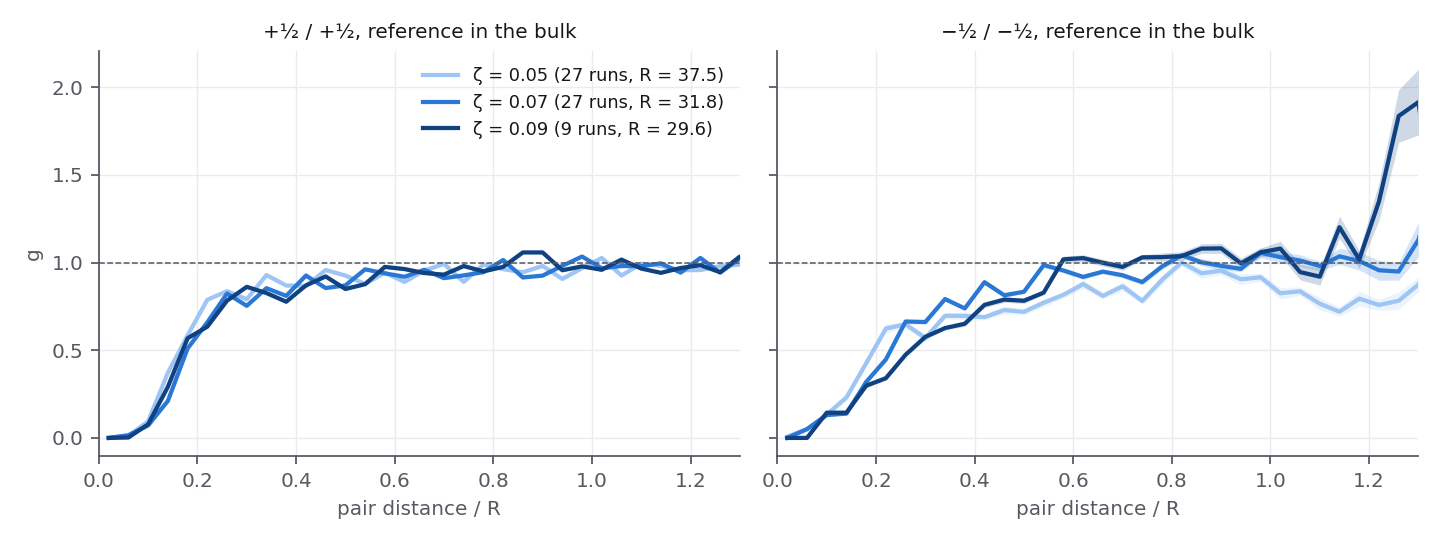
\includegraphics[width=0.85\textwidth]{g_act.png}
\caption{Bulk pair correlations at $\zeta=0.05$, 0.07, 0.09 in units of $r/R$ ($R=1.43\,\la$ at each activity).}\label{fig:gact}
\end{figure}
\paragraph{Density stratification.} \SIcand The vortex centrifuges particles towards the wall (compressibility, Mach number
$\sim1$). In cavities with $k=8$ at the activity-scan radii:
\begin{table}[H]\centering\small
\caption{Particle occupancy per cell ($\langle n\rangle=20$; Poisson standard deviation 4.47), by distance $s$ from the wall.}\label{tab:dens}
\begin{adjustbox}{max width=\textwidth}
\begin{tabular}{lcccccc}\toprule
$\zeta$ & SD / Poisson & $s<5$ & centre $s>20$ & $P(n<10)$ all & $P(n<10)$ centre & $-\half$ cores\\\midrule
0.07 & 1.5 & 25 & 14 & 4.5\% & 15\% & 15\\
0.09 & 2.0 & 28 & 9 & 15\% & 60\% & 11\\
0.11 & 2.2 & 29 & 8 & 17\% & 70\% & 11\\\bottomrule
\end{tabular}
\end{adjustbox}
\end{table}
The gap region ($s=3$--5) is over-dense (25--28), so low occupancy does not explain the closing gap. Even at $\zeta=0.07$ the
centre is depleted by $\approx30\%$; $-\half$ cores sit in depleted cells. collOp 21 is a density-modulated dipole, so the active
stress varies with this stratification. This is a property of particle-based active nematics at finite Mach number and should
be stated in the methods; a low-Mach control (higher $k_BT$) would change the whole calibration and is not planned.
